\subsection{Telepítés}
\subsubsection{Java SE Runtime Environment 8}
A programcsomag futtatásához legalább Windows XP operációs rendszer szükséges, amelyen Java SE Runtime Environment 8 futtató környezet \cite{jresite} (a továbbiakban: JRE) fut. A JRE feltelepítését követően manuálisan ellenőrizzük, hogy a rendszer felvette-e környezeti változóként az installációs könyvtárat. Navigáljunk az operációs rendszerben a környezeti változók módosítása panelhez, majd ellenőrizzük le, hogy a PATH nevű környezeti változóhoz hozzá lett-e adva az installációs könyvtár: \path{C:\Program Files\Java\jdk1.8.0_60\bin}. 
Ha nem, akkor pontosvesszővel (;) elválasztva egészítsük ki a változó értékét, majd indítsuk el a promptot (ha nyitva van, akkor indítsuk újra).
Ha a
\begin{verbatim}
java -version
\end{verbatim}
utasítás hatására az 
\begin{figure}[h!]
  \caption{JRE verzió}
  \label{fig:jre_version}
  \centering
    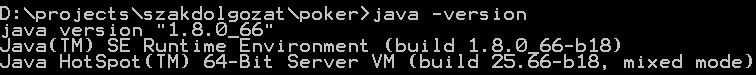
\includegraphics{user-documentation/images/java_version.jpg}
\end{figure}
 \ref{fig:jre_version}. ábrán látható szöveg jelenik meg a konzolon, akkor sikeres volt a JRE telepítése és beállítása. További instrukciókért ld. melléklet.
 
 \subsubsection{MySQL Community Server 5.6}
 A programcsomag megköveteli a MySQL Community Server 5.6 adatbázis-kezelő rendszer \cite{mysqlsite} (a továbbiakban: MySQL Server) használatát is. Letöltés után csomagoljuk ki a zip állományt egy tetszőleges könyvtárba, majd a fentiekkel megegyező módon adjuk hozzá a PATH nevű környezeti változó értékéhez a MySQL Server bin könyvtár elérési útvonalát. Ha ezzel végeztünk, akkor nyissük meg a promptot (ha nyitva van, akkor indítsuk újra), majd navigáljunk a MySQL Server bin könyvtárába, ott pedig adjuk ki a
 \begin{verbatim}
mysqld --install
\end{verbatim}
parancsot. A parancs végrehajtása után navigáljunk a szolgáltatások panelhez, amelyet a legkönnyebben a promptban a
 \begin{verbatim}
services.msc
\end{verbatim}
\begin{figure}[h!]
  \caption{MySQL Service}
  \label{fig:mysql_service}
  \centering
    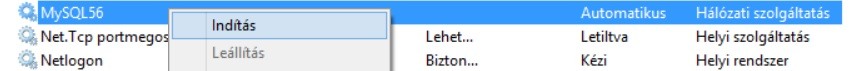
\includegraphics{user-documentation/images/mysql_service.jpg}
\end{figure}
kiadott utasítással lehet elérni. Majd járjunk el a \ref{fig:mysql_service}. ábrának megfelelően. Térjünk vissza a konzolra, ahol adjuk ki a 
 \begin{verbatim}
mysql -u root -p
\end{verbatim}
parancsot, amely jelszót fog kérni. A beviteli sort hagyjuk üresen, nyomjunk entert. Ha sikeresen beléptünk az adatbázis-kezelő rendszerbe, akkor adjuk ki a
 \begin{verbatim}
SELECT VERSION();
\end{verbatim}
utasítást, és ha a 
\begin{figure}[h!]
  \caption{MySQL Service}
  \label{fig:mysql_service}
  \centering
    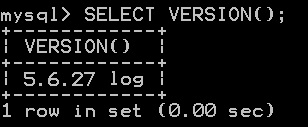
\includegraphics{user-documentation/images/mysql_version.jpg}
\end{figure}
\ref{fig:mysql_service}. ábrának megfelelő képernyőképet kapunk, akkor sikeresen feltelepítettük az adatbázis-kezelő rendszert.

\subsubsection{Az adatbázis használatba vétele}
Ha sikeresen elindítottuk a MySQL Servert, akkor szükségünk lesz egy új adatbázis sémára (és demo adatokra), amelyet a \path{X:\poker\release\poker-db.sql} állományban találunk. Ezt a filet kell lefuttatni az adatbázison, a hatása idempotens. A promptban adjuk ki a
 \begin{verbatim}
mysql -u root -p < X:\poker\release\poker-db.sql
\end{verbatim}
utasítást, amely jelszót fog kérni. A beviteli sort ugyancsak hagyjuk üresen. Ha sikeresen lefutott a parancs, akkor az adatbázis séma ``felhúzása'' megtörtént.

\subsubsection{A póker szerver elindítása}
A DVD lemezen a \path{\poker\release\} mappában található meg a poker-server-1.0.0.jar file. Nyissunk egy terminált a kijelölt könyvtárban, és adjuk ki a
 \begin{verbatim}
java -jar poker-server-1.0.0.jar
\end{verbatim}
parancsot. 
\begin{figure}[h!]
  \caption{Szerver}
  \label{fig:server_started}
  \centering
    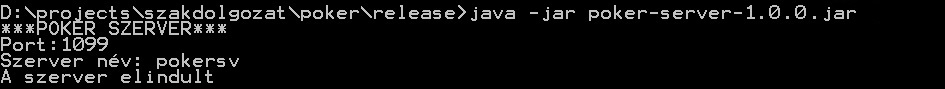
\includegraphics{user-documentation/images/server_started.jpg}
\end{figure}
Ha a \ref{fig:server_started}. ábrának megfelelő konzol loglistát látunk, akkor a szervert sikeresen elindítottuk.
\subsubsection{A póker kliens elindítása}
A kliens futtatása hasonló módon történik, mint a szerveré. Navigáljunk a \path{\release\poker\kliens} mappába, és a konzolon adjuk ki a megfeleő parancsot.
Jöhet az ábra, meg a kódot kicsit átírni, hogy logoljon konzolra, mint a szerver...
\subsection{Futtatás}
A program java programozási nyelvben lett megírva, így a kifordított állomány egy jar file, melyet parancssorból az alábbi utasítással tudunk futtatni
\begin{lstlisting}
java -jar <filenev>
\end{lstlisting}
\subsection{Felhasznált technológiák}
A szakdolgozatomat eclipse fejlesztőkörnyezetben írtam, amelyet végül mavennel fordítottam ki és csomagoltam be. A szakdolgozat felhasznál egy külső könyvtárat \cite{hand_eval}, amely a nyertes kiértékelési feladatát látja el. A programcsomagot meg kellett támogatni egy adatbázissal is - MySQL - , amely az adatok perzisztens tárolásáért felel. A programcsomag szerver-kliens architektúrában került implementálásra, amely tovább bomlik kliens oldalon MVC (Model-View-Controller) tervezési stílusra. A modulok közötti kommunikáció RMI Java API felhasználásával történik.
\subsection{Adatbázis séma}
\begin{figure}[h!]
  \caption{Adatbázis séma}
  \centering
    \includegraphics[width=0.5\textwidth]{user-documentation/images/db_scheme.png}
\end{figure}
Az
\subsection{Modulok}
A programcsomag 6 fő modult tartalmaz
\begin{itemize}
  \item poker-server
  A póker játék szervere, amely magát a játékot szolgáltatja.
  \item poker-client
  A póker játék kliense, amely segítségével a szerverhez lehet csatlakozni.
  \item poker-shared
  A póker játék azon modulja, amelytől a szerver és a kliens egyaránt függ.
  \item poker-persist
  Az adatok letárolásáért felelős modul.
  \item poker-model
  A póker játék modellezéséért felelős csomag.
  \item javapokertexasholdem
  Külső könyvtár, amely a nyertes játékos kiértékelési feladatot végzi.
\end{itemize}
\begin{figure}[h!]
	\caption{Kliens modulra bontása}
	\centering
	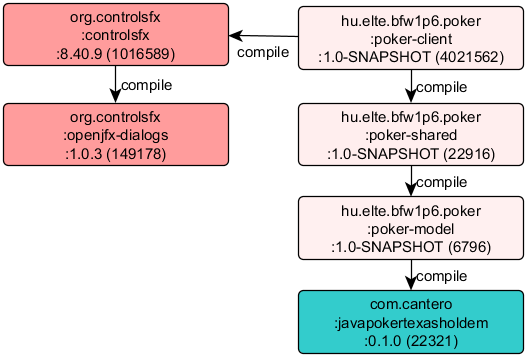
\includegraphics{user-documentation/images/poker-client-deps.png}
\end{figure}
\begin{figure}[h!]
	\caption{Szerver modulra bontása}
	\centering
	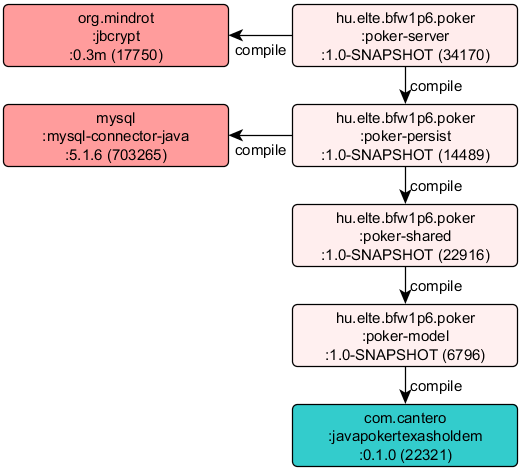
\includegraphics{user-documentation/images/poker-server-deps.png}
\end{figure}
A modulok közötti függőséget a ... ábra mutatja. A programcsomag két fő modulra bontható: poker-server és poker-client. A szerver a jelszavak titkosítására bcrypt eljárást alkalmaz, amelynek a biztonságát sózással növeli. Továbbá a szerver felhasznál még egy külső csomagot - mysql-connector-java -, amely az adatbázis kapcsolatért felel.
A poker-shared modul felel a szerver és a kliens jól definiált kommunikácójáért. A shared modul többek között tartalmazza a közös interfészeket, kivételeket és a póker utasítások megvalósítását. A kliens közvetlenül függ ettől a modultól, azonban a szerver és a shared modul közé beékelődött a poker-persist modul.

\section{Funkciók}
Ahogy a témabejelentőben is szerepel...... RMI kép wikiről, majd azt megmagyarázni a shared modullal, kliens hívja, jól definiált interfész etc....
\begin{figure}[h!]
	\caption{RMI koncepció}
	\centering
	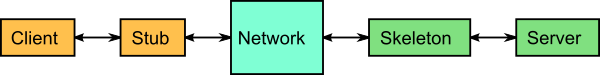
\includegraphics[width=14cm, height=2cm]{user-documentation/images/rmi.png}
\end{figure}
A szerver vázáért a PokerRemote interface felel, amely a játékon végrehajtható műveletek összefogásáért felel. Itt található az összes funkció, amely megvalósításra került, mint például játék asztal létrehozása, új felhasználó létrehozás, admin jog kiosztása stb. A kliens ezt a vázat tudja elkérni a registryből, mint kliens-oldali szervercsonk, amelyeken a műveletek meg tudja hívni. Az összes megvalósított funkciót le kell írni? Felsorolás szintjén, vagy hogy? Rövid magyarázattal? És amelyik egyértelmű? Pl. felhasználó módosítása... login...

\section{Tovább fejlesztési lehetőségek}
\begin{itemize}
\item Az adatbázis viszonylag alacsony absztrakciós szinten került implementására, azonban mivel néhány tábláról beszélhetünk csak, ezért igyekeztem elkerülni a keretrendszerek általi overheadet. Ugyanakkor ezen a ponton sokat fejlődhet a programcsomag, ha a későbbiek során esetlegesen bonyolultabban kellene modellezni a játékot adatbázis szempontjából. Például dialektusok - akár Liquibase (hivatkozás) - használata elfedheti a tényleges adatbázis-kezelő rendszer általánosságait, így eggyel magasabb szintre helyezhető a megvalósítás.
\item A felhasználói élményen sokat javíthat az animációk használata. A megjelenítés sokkal lágyabb, folyékonyabb lehetne Transition/Animation (bibliográfiába hivatkozás...) objektumok használatával.
\item Akár a komplett RMI architektúrát (JDK 1.1-ben jelent meg 18 éves technológia [a http meg 16...]) le lehetne váltani, és helyette REST szoftverarchitektúrát tenni, amely modernebb megjelenést (AngularJS, reszponzív design) és modernebb eszközöket vonna maga után.
\end{itemize}

%\begin{figure}[hbt]
%	\centering
%	\includegraphics[width=\linewidth, height=8cm]{db_scheme.png}
%	\caption{Adatbázis séma}
%	\label{fig:lol}
%\end{figure}

A \ref{fig:lol} képen látható az adatbázis séma.
\section{Tesztelés}
\subsection{Funkcionális tesztelés}
\begin{tabular}{| l | c | r |}
\hline
  Funkció & Elvárt eredmény & eredmény \\ \hline
  Regisztráció & A program jelezte a felhasználónak, hogy a regisztráció sikeresen megtörtént, és visszairányította őt a bejelentkezési formhoz. & A felhasználó a regisztrációt követően be tudjon jelentkezni a póker játékba. \\ \hline
  Bejelentkezés & A formot helyesen kitöltve a program sikeresen autentikálta és beléptette a felhasználót. & Regisztrációt követően be tudjon jelentkezni a felhasználó \\ \hline
  Tábla módosítás & - & - \\ \hline
  Tábla törlés & - & - \\ \hline
\end{tabular}

\clearpage
